\begin{figure}
\centering
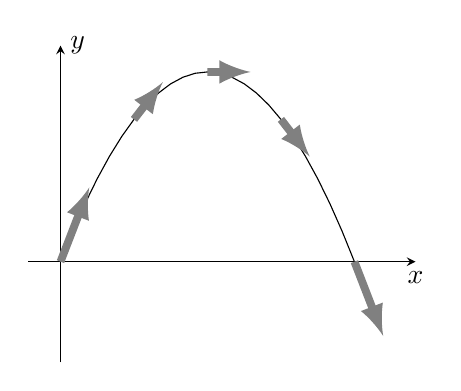
\begin{tikzpicture}[declare function={fx(\t)=\t;fy(\t)=\t-9.8/2*\t^2;gx(\t)=1;gy(\t)=1-9.8*\t;}]
\pgfmathsetmacro{\ta}{0.0*2/9.8}
\pgfmathsetmacro{\tb}{0.25*2/9.8}
\pgfmathsetmacro{\tc}{0.5*2/9.8}
\pgfmathsetmacro{\td}{0.75*2/9.8}
\pgfmathsetmacro{\te}{1.0*2/9.8}
\begin{axis}[clip=false,view/h=110,small,axis lines=middle,xtick={\empty},ytick={\empty},ztick={\empty},enlargelimits=true, xlabel={$x$}, ylabel={$y$},zlabel={$z$}, xlabel style={anchor=north},ylabel style={anchor=west},zlabel style={anchor=south},colormap={}{gray(0cm)=(0.6);gray(1cm)=(0.9);}]
\addplot[domain=0:2/9.8,variable =\t] ({fx(t)},{fy(t)});
\addplot[-latex,line width=1mm, gray]plot coordinates {({fx(\ta)},{fy(\ta)})({fx(\ta)+0.02*gx(\ta)},{fy(\ta)+0.02*gy(\ta)})};
\addplot[-latex,line width=1mm, gray]plot coordinates {({fx(\tb)},{fy(\tb)})({fx(\tb)+0.02*gx(\tb)},{fy(\tb)+0.02*gy(\tb)})};
\addplot[-latex,line width=1mm, gray]plot coordinates {({fx(\tc)},{fy(\tc)})({fx(\tc)+0.03*gx(\tc)},{fy(\tc)+0.02*gy(\tc)})};
\addplot[-latex,line width=1mm, gray]plot coordinates {({fx(\td)},{fy(\td)})({fx(\td)+0.02*gx(\td)},{fy(\td)+0.02*gy(\td)})};
\addplot[-latex,line width=1mm, gray]plot coordinates {({fx(\te)},{fy(\te)})({fx(\te)+0.02*gx(\te)},{fy(\te)+0.02*gy(\te)})};
\end{axis}
\end{tikzpicture}
\caption{گول انداز کے سمتی رفتار سمتیات \عددی{\kvec{v}(t)} سمتی میدان دیتے ہیں۔}
\label{شکل_سمتی_تکمل_سمتی_رفتار_میدان}
\end{figure}


\begin{figure}
\centering
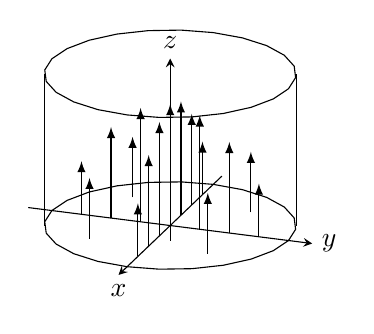
\begin{tikzpicture}[declare function={fx(\t)=cos(\t);fy(\t)=sin(\t);gz(\x,\y)=1-\x^2-\y^2;}]
\begin{axis}[clip=false,view/h=110,small,axis lines=middle,xtick={\empty},ytick={\empty},ztick={\empty},enlargelimits=true, xlabel={$x$}, ylabel={$y$},zlabel={$z$}, xlabel style={anchor=north},ylabel style={anchor=west},zlabel style={anchor=south},colormap={}{gray(0cm)=(0.6);gray(1cm)=(0.9);}]
\addplot3[domain=0:360,variable =\t] ({fx(t)},{fy(t)},{0});
\addplot3[domain=0:360,variable =\t] ({fx(t)},{fy(t)},{1.25});
\addplot3[]plot coordinates {({fx(110)},{fy(110)},{0})({fx(110)},{fy(110)},{1.25})};
\addplot3[]plot coordinates {({fx(110+180)},{fy(110+180)},{0})({fx(110+180)},{fy(110+180)},{1.25})};
\addplot3[-latex]plot coordinates {(0,0,0)(0,0,{gz(0,0)})};
\addplot3[-latex]plot coordinates {(-0.25,0,0)(-0.25,0,{gz(-0.25,0)})};
\addplot3[-latex]plot coordinates {(-0.5,0,0)(-0.5,0,{gz(-0.5,0)})};
\addplot3[-latex]plot coordinates {(-0.75,0,0)(-0.75,0,{gz(-0.75,0)})};
\addplot3[-latex]plot coordinates {(0.25,0,0)(00.25,0,{gz(0.25,0)})};
\addplot3[-latex]plot coordinates {(0.5,0,0)(00.5,0,{gz(0.5,0)})};
\addplot3[-latex]plot coordinates {(0.75,0,0)(00.75,0,{gz(0.75,0)})};
%
\addplot3[-latex]plot coordinates {(0,-0.25,0)(0,-0.25,{gz(0,-0.25)})};
\addplot3[-latex]plot coordinates {(0,-0.5,0)(0,-0.5,{gz(0,-0.5)})};
\addplot3[-latex]plot coordinates {(0,-0.75,0)(0,-0.75,{gz(0,-0.75)})};
\addplot3[-latex]plot coordinates {(0,0.25,0)(0,0.25,{gz(0,0.25)})};
\addplot3[-latex]plot coordinates {(0,0.5,0)(0,0.5,{gz(0,0.5)})};
\addplot3[-latex]plot coordinates {(0,0.75,0)(0,0.75,{gz(0,0.75)})};
%
\addplot3[-latex]plot coordinates {(-0.5,-0.5,0)(-0.5,-0.5,{gz(-0.5,-0.5)})};
\addplot3[-latex]plot coordinates {(0.5,-0.5,0)(0.5,-0.5,{gz(0.5,-0.5)})};
\addplot3[-latex]plot coordinates {(0.5,0.5,0)(0.5,0.5,{gz(0.5,0.5)})};
\addplot3[-latex]plot coordinates {(-0.5,0.5,0)(-0.5,0.5,{gz(-0.5,0.5)})};
\end{axis}
\end{tikzpicture}
\caption{
لمبی نالی میں سیال کی حرکت۔ مستوی \عددی{xy} میں  سمتیات \عددی{\kvec{v}=(a^2-\rho^2)\ak} کی دم اور قطع مکافی \عددی{z=a^2-\rho^2} پر  سر پائے جاتے ہیں۔
}
\label{شکل_سمتی_تکمل_نلکی_میں_بہاو_سیال}
\end{figure}



\begin{figure}
\centering
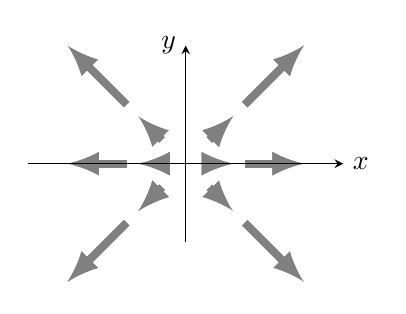
\begin{tikzpicture}[declare function={fx(\x,\y)=\x;fy(\x,\y)=\y;}]
\pgfmathsetmacro{\ka}{0.3}
\draw[-latex,gray,line width=1mm](\ka,0)--++({fx(\ka,0)},{fy(\ka,0)});
\draw[-latex,gray,line width=1mm](\ka,\ka)--++({fx(\ka,\ka)},{fy(\ka,\ka)});
\draw[-latex,gray,line width=1mm](\ka,0)--++({fx(\ka,0)},{fy(\ka,0)});
\draw[-latex,gray,line width=1mm](\ka,\ka)--++({fx(\ka,\ka)},{fy(\ka,\ka)});
\pgfmathsetmacro{\ka}{0.75}
\draw[-latex,gray,line width=1mm](\ka,0)--++({fx(\ka,0)},{fy(\ka,0)});
\draw[-latex,gray,line width=1mm](\ka,\ka)--++({fx(\ka,\ka)},{fy(\ka,\ka)});
\draw[-latex,gray,line width=1mm](\ka,0)--++({fx(\ka,0)},{fy(\ka,0)});
\draw[-latex,gray,line width=1mm](\ka,\ka)--++({fx(\ka,\ka)},{fy(\ka,\ka)});
\pgfmathsetmacro{\ka}{-0.3}
\draw[-latex,gray,line width=1mm](\ka,0)--++({fx(\ka,0)},{fy(\ka,0)});
\draw[-latex,gray,line width=1mm](\ka,\ka)--++({fx(\ka,\ka)},{fy(\ka,\ka)});
\draw[-latex,gray,line width=1mm](\ka,0)--++({fx(\ka,0)},{fy(\ka,0)});
\draw[-latex,gray,line width=1mm](\ka,\ka)--++({fx(\ka,\ka)},{fy(\ka,\ka)});
\pgfmathsetmacro{\ka}{-0.75}
\draw[-latex,gray,line width=1mm](\ka,0)--++({fx(\ka,0)},{fy(\ka,0)});
\draw[-latex,gray,line width=1mm](\ka,\ka)--++({fx(\ka,\ka)},{fy(\ka,\ka)});
\draw[-latex,gray,line width=1mm](\ka,0)--++({fx(\ka,0)},{fy(\ka,0)});
\draw[-latex,gray,line width=1mm](\ka,\ka)--++({fx(\ka,\ka)},{fy(\ka,\ka)});
\pgfmathsetmacro{\ka}{0.3}
\draw[-latex,gray,line width=1mm](\ka,-\ka)--++({fx(\ka,-\ka)},{fy(\ka,-\ka)});
\pgfmathsetmacro{\ka}{-0.3}
\draw[-latex,gray,line width=1mm](\ka,-\ka)--++({fx(\ka,-\ka)},{fy(\ka,-\ka)});
\pgfmathsetmacro{\ka}{0.75}
\draw[-latex,gray,line width=1mm](\ka,-\ka)--++({fx(\ka,-\ka)},{fy(\ka,-\ka)});
\pgfmathsetmacro{\ka}{-0.75}
\draw[-latex,gray,line width=1mm](\ka,-\ka)--++({fx(\ka,-\ka)},{fy(\ka,-\ka)});
\draw[-stealth](-2,0)--(2,0)node[right]{$x$};
\draw[-stealth](0,-1)--(0,1.5)node[left]{$y$};
\end{tikzpicture}
\caption{
مستوی میں مختلف نقاط پر  رداسی میدان \عددی{\kvec{F}=x\ai+y\aj} جہاں تیر دار لکیر کی دم اس نقطہ پر رکھی جاتی ہے جہاں کا سمتیہ درکار ہو۔
}
\label{شکل_سمتی_تکمل_رداسی_میدان}
\end{figure}

